\begin{figure}[t]
\centering
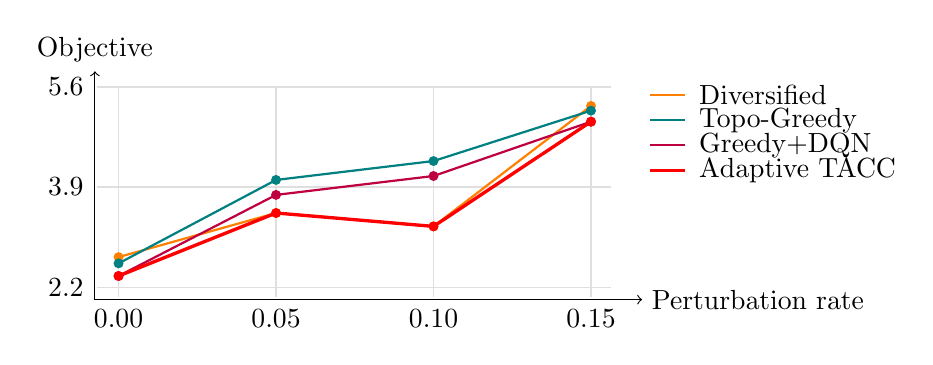
\begin{tikzpicture}[x=1cm,y=1cm]
\draw[->] (0.7,0.55) -- (7.65,0.55) node[right] {Perturbation rate};
\draw[->] (0.7,0.55) -- (0.7,3.45) node[above] {Objective};
\node[below] at (1.00,0.55) {0.00};
\draw[gray!25] (1.00,0.58) -- (1.00,3.25);
\node[below] at (3.00,0.55) {0.05};
\draw[gray!25] (3.00,0.58) -- (3.00,3.25);
\node[below] at (5.00,0.55) {0.10};
\draw[gray!25] (5.00,0.58) -- (5.00,3.25);
\node[below] at (7.00,0.55) {0.15};
\draw[gray!25] (7.00,0.58) -- (7.00,3.25);
\draw[gray!25] (0.72,0.70) -- (7.25,0.70);
\node[left] at (0.68,0.70) {2.2};
\draw[gray!25] (0.72,1.98) -- (7.25,1.98);
\node[left] at (0.68,1.98) {3.9};
\draw[gray!25] (0.72,3.25) -- (7.25,3.25);
\node[left] at (0.68,3.25) {5.6};
\draw[orange, thick] (1.00,1.09) -- (3.00,1.65) -- (5.00,1.48) -- (7.00,3.01);
\fill[orange] (1.00,1.09) circle (1.8pt);
\fill[orange] (3.00,1.65) circle (1.8pt);
\fill[orange] (5.00,1.48) circle (1.8pt);
\fill[orange] (7.00,3.01) circle (1.8pt);
\draw[orange, thick] (7.75,3.15) -- (8.20,3.15);
\node[right] at (8.25,3.15) {Diversified};
\draw[teal, thick] (1.00,1.01) -- (3.00,2.07) -- (5.00,2.31) -- (7.00,2.95);
\fill[teal] (1.00,1.01) circle (1.8pt);
\fill[teal] (3.00,2.07) circle (1.8pt);
\fill[teal] (5.00,2.31) circle (1.8pt);
\fill[teal] (7.00,2.95) circle (1.8pt);
\draw[teal, thick] (7.75,2.83) -- (8.20,2.83);
\node[right] at (8.25,2.83) {Topo-Greedy};
\draw[purple, thick] (1.00,0.85) -- (3.00,1.88) -- (5.00,2.12) -- (7.00,2.81);
\fill[purple] (1.00,0.85) circle (1.8pt);
\fill[purple] (3.00,1.88) circle (1.8pt);
\fill[purple] (5.00,2.12) circle (1.8pt);
\fill[purple] (7.00,2.81) circle (1.8pt);
\draw[purple, thick] (7.75,2.51) -- (8.20,2.51);
\node[right] at (8.25,2.51) {Greedy+DQN};
\draw[red, very thick] (1.00,0.85) -- (3.00,1.65) -- (5.00,1.48) -- (7.00,2.81);
\fill[red] (1.00,0.85) circle (1.8pt);
\fill[red] (3.00,1.65) circle (1.8pt);
\fill[red] (5.00,1.48) circle (1.8pt);
\fill[red] (7.00,2.81) circle (1.8pt);
\draw[red, very thick] (7.75,2.19) -- (8.20,2.19);
\node[right] at (8.25,2.19) {Adaptive TACC};
\end{tikzpicture}
\caption{Objective trends for the strongest placement policies across perturbation rates. Adaptive TACC follows the best regime-specific candidate rather than forcing one static policy.}
\label{fig:generated_objective_trends}
\end{figure}
